\documentclass[aspectratio=169, 10pt]{beamer}

% ── Theme ─────────────────────────────────────────────────────────────────────
\usetheme{Madrid}
\usecolortheme{default}
\usefonttheme{professionalfonts}
\setbeamertemplate{navigation symbols}{}
\setbeamertemplate{footline}[frame number]

% ── Packages ──────────────────────────────────────────────────────────────────
\usepackage[T1]{fontenc}
\usepackage[utf8]{inputenc}
\usepackage{lmodern}
\usepackage{microtype}
\usepackage{graphicx}
\usepackage{booktabs}
\usepackage{array}
\usepackage{tabularx}
\usepackage{amsmath}
\usepackage{listings}
\usepackage{tikz}
\usetikzlibrary{shapes.geometric, arrows.meta, positioning, fit, backgrounds, calc}
\usepackage{xcolor}

% ── Colours ───────────────────────────────────────────────────────────────────
\definecolor{umons-blue}{HTML}{003366}
\definecolor{umons-light}{HTML}{E8EEF5}
\definecolor{asp-green}{HTML}{27AE60}
\definecolor{t-blue}{HTML}{3498DB}
\definecolor{l-red}{HTML}{E74C3C}
\definecolor{plus-purple}{HTML}{9B59B6}
\definecolor{code-bg}{HTML}{F4F6F9}
\definecolor{code-border}{HTML}{BDC3C7}
\definecolor{piece-I}{HTML}{E74C3C}
\definecolor{piece-T}{HTML}{3498DB}
\definecolor{piece-L}{HTML}{2ECC71}
\definecolor{piece-Pyr}{HTML}{9B59B6}
\definecolor{piece-O}{HTML}{F39C12}
\definecolor{piece-N}{HTML}{F1C40F}
\definecolor{piece-Z}{HTML}{1ABC9C}
\definecolor{piece-Zm}{HTML}{E91E63}
\definecolor{hint-gold}{HTML}{F39C12}

% ── Beamer colour overrides ───────────────────────────────────────────────────
\setbeamercolor{palette primary}{bg=umons-blue, fg=white}
\setbeamercolor{palette secondary}{bg=umons-blue!80, fg=white}
\setbeamercolor{palette tertiary}{bg=umons-blue!60, fg=white}
\setbeamercolor{palette quaternary}{bg=umons-blue, fg=white}
\setbeamercolor{structure}{fg=umons-blue}
\setbeamercolor{section in toc}{fg=umons-blue}
\setbeamercolor{block title}{bg=umons-blue, fg=white}
\setbeamercolor{block body}{bg=umons-light}
\setbeamercolor{alerted text}{fg=l-red}
\setbeamercolor{example text}{fg=asp-green}

% ── Beamer font ───────────────────────────────────────────────────────────────
\setbeamerfont{title}{size=\large, series=\bfseries}
\setbeamerfont{frametitle}{size=\normalsize, series=\bfseries}

% ── Speaker label command ─────────────────────────────────────────────────────
\newcommand{\abdelhadi}{%
  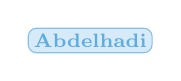
\begin{tikzpicture}[baseline=-2pt]
    \node[rounded corners=3pt, fill=t-blue!20, draw=t-blue!60,
          inner sep=2pt, font=\scriptsize\bfseries, text=t-blue!80] {Abdelhadi};
  \end{tikzpicture}}
\newcommand{\mohamed}{%
  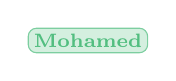
\begin{tikzpicture}[baseline=-2pt]
    \node[rounded corners=3pt, fill=asp-green!20, draw=asp-green!60,
          inner sep=2pt, font=\scriptsize\bfseries, text=asp-green!80] {Mohamed};
  \end{tikzpicture}}

% ── TikZ unit square macro --- defined in preamble to avoid Beamer # conflict ──
\newcommand{\sqfill}[3]{%  \sqfill{x}{y}{color}
  \fill[#3, draw=black, line width=0.4pt] (#1,#2) rectangle +(1,1);}

% ── ASP listing style ─────────────────────────────────────────────────────────
\lstdefinelanguage{ASP}{
  keywords={not, true, false},
  keywordstyle=\color{umons-blue}\bfseries,
  morecomment=[l]{\%},
  commentstyle=\color{gray!70}\itshape,
  stringstyle=\color{l-red},
  morestring=[b]",
  sensitive=true,
  basicstyle=\ttfamily\scriptsize,
  breaklines=true,
}
\lstdefinestyle{aspstyle}{
  language=ASP,
  backgroundcolor=\color{code-bg},
  frame=single,
  framerule=0.5pt,
  rulecolor=\color{code-border},
  xleftmargin=4pt, xrightmargin=4pt,
}
\lstdefinestyle{bashstyle}{
  language=bash,
  backgroundcolor=\color{umons-blue!8},
  basicstyle=\ttfamily\scriptsize,
  frame=single,
  framerule=0.5pt,
  rulecolor=\color{umons-blue!30},
  xleftmargin=4pt, xrightmargin=4pt,
  breaklines=true,
}

% ── Title info ────────────────────────────────────────────────────────────────
\title[Tetracube Puzzles with ASP]{%
  Generating and Solving 3D Tetracube Puzzles\\
  in Arbitrary Non-Rectangular Volumes with ASP}
\author[Agourzam \& El ismaily]{%
  Abdelhadi Agourzam \and Mohamed El ismaily}
\institute[UMONS]{%
  Université de Mons (UMONS), Faculté des Sciences\\
  Knowledge Representation and Reasoning, 2026}
\date{May 2026}

% ─────────────────────────────────────────────────────────────────────────────
\begin{document}

% ══════════════════════════════════════════════════════════════════════════════
% TITLE SLIDE
% ══════════════════════════════════════════════════════════════════════════════
\begin{frame}[plain]
  \begin{tikzpicture}[remember picture, overlay]
    \fill[umons-blue] (current page.north west)
          rectangle ([yshift=-3.2cm]current page.north east);
    \fill[t-blue!70] ([yshift=-3.2cm]current page.north west)
          rectangle ([yshift=-3.7cm]current page.north east);
    \node[anchor=west, text=white, font=\large\bfseries]
          at ([xshift=1.2cm, yshift=-1.3cm]current page.north west)
          {Final Presentation};
    \node[anchor=west, text=white!80, font=\small]
          at ([xshift=1.2cm, yshift=-2.0cm]current page.north west)
          {Knowledge Representation and Reasoning, 2026};
    \node[anchor=west, text=white!60, font=\footnotesize]
          at ([xshift=1.2cm, yshift=-2.7cm]current page.north west)
          {Université de Mons (UMONS) --- Faculté des Sciences};
  \end{tikzpicture}

  \vspace{3.6cm}

  {\color{umons-blue}\Large\bfseries
    Generating and Solving 3D Tetracube Puzzles\\[0.2cm]
    in Arbitrary Non-Rectangular Volumes with ASP}

  \vspace{0.3cm}
  {\color{umons-blue!50}\rule{\linewidth}{1pt}}
  \vspace{0.3cm}

  \begin{columns}[T]
    \column{0.55\textwidth}
      \textbf{Authors:} Abdelhadi Agourzam \quad|\quad Mohamed El ismaily\\[4pt]
      \textbf{Supervisor:} Jef Wijsen \quad\textbf{Date:} May 2026

    \column{0.42\textwidth}
      \centering
      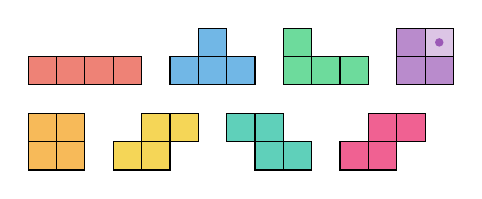
\begin{tikzpicture}[scale=0.36]
        % Row 1: I T L Pyramid
        \sqfill{0}{0}{piece-I!70}\sqfill{1}{0}{piece-I!70}
        \sqfill{2}{0}{piece-I!70}\sqfill{3}{0}{piece-I!70}
        %
        \sqfill{5}{0}{piece-T!70}\sqfill{6}{0}{piece-T!70}
        \sqfill{7}{0}{piece-T!70}\sqfill{6}{1}{piece-T!70}
        %
        \sqfill{9}{0}{piece-L!70}\sqfill{10}{0}{piece-L!70}
        \sqfill{11}{0}{piece-L!70}\sqfill{9}{1}{piece-L!70}
        %
        \sqfill{13}{0}{piece-Pyr!70}\sqfill{14}{0}{piece-Pyr!70}
        \sqfill{13}{1}{piece-Pyr!70}
        \fill[piece-Pyr!35, draw=black, line width=0.3pt]
              (14,1) rectangle +(1,1);
        \fill[piece-Pyr] (14.5,1.5) circle (0.15);
        % Row 2: O N Z Zm
        \sqfill{0}{-3}{piece-O!70}\sqfill{1}{-3}{piece-O!70}
        \sqfill{0}{-2}{piece-O!70}\sqfill{1}{-2}{piece-O!70}
        %
        \sqfill{3}{-3}{piece-N!70}\sqfill{4}{-3}{piece-N!70}
        \sqfill{4}{-2}{piece-N!70}\sqfill{5}{-2}{piece-N!70}
        %
        \sqfill{7}{-2}{piece-Z!70}\sqfill{8}{-2}{piece-Z!70}
        \sqfill{8}{-3}{piece-Z!70}\sqfill{9}{-3}{piece-Z!70}
        %
        \sqfill{11}{-3}{piece-Zm!70}\sqfill{12}{-3}{piece-Zm!70}
        \sqfill{12}{-2}{piece-Zm!70}\sqfill{13}{-2}{piece-Zm!70}
      \end{tikzpicture}
  \end{columns}
\end{frame}

% ══════════════════════════════════════════════════════════════════════════════
% PART 1
% ══════════════════════════════════════════════════════════════════════════════

\begin{frame}[plain]
  \begin{tikzpicture}[remember picture, overlay]
    \fill[umons-blue!90] (current page.center) circle (4.5cm);
    \node[text=white, font=\LARGE\bfseries, align=center]
          at (current page.center)
          {Part 1\\[8pt]\Large The Problem \& The Pieces};
  \end{tikzpicture}
\end{frame}

% ── Slide 1 ───────────────────────────────────────────────────────────────────
\begin{frame}{Slide 1 --- Introduction \hfill \abdelhadi}
  \begin{columns}[T]
    \column{0.42\textwidth}
      \begin{block}{What is a Tetracube?}
        {\small A 3D figure of \textbf{4 unit cubes} joined face-to-face.
        \textbf{8 distinct} types $\Rightarrow$
        $8\times4=\mathbf{32}$ unit cubes total.}
      \end{block}

      \vspace{0.15cm}
      \begin{alertblock}{The Core Question}
        {\small Can all 8 pieces pack into \textbf{non-rectangular}
        3D volumes using a \emph{single, unmodified} ASP engine?}
      \end{alertblock}

      \vspace{0.15cm}
      \begin{exampleblock}{Our Answer}
        {\small \textbf{Yes} --- any connected 32-cell volume works.\\
        One predicate: \texttt{cell(X,Y,Z)}.}
      \end{exampleblock}

      \vspace{0.15cm}
      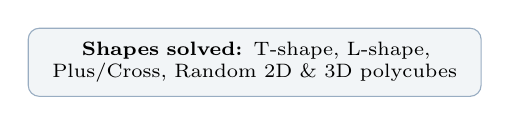
\begin{tikzpicture}
        \node[draw=umons-blue!40, fill=umons-blue!5, rounded corners=4pt,
              text width=5.4cm, align=center, font=\scriptsize, inner sep=5pt]{%
          \textbf{Shapes solved:} T-shape, L-shape,\\
          Plus/Cross, Random 2D \& 3D polycubes};
      \end{tikzpicture}

    \column{0.55\textwidth}
      \centering
      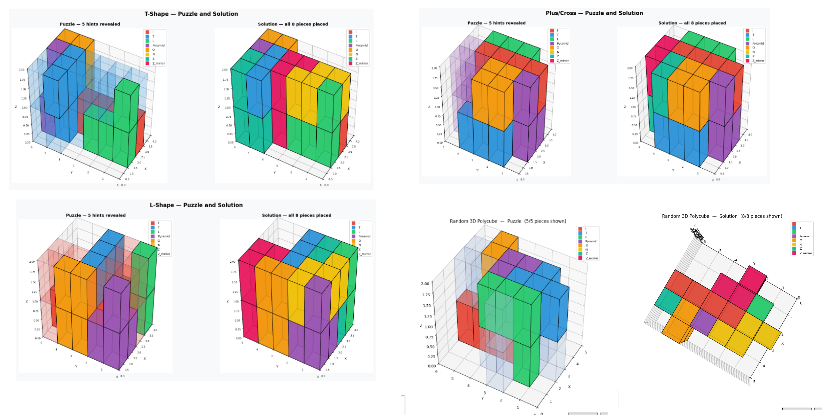
\includegraphics[width=\linewidth]{img_overview}
      {\scriptsize\color{gray} Puzzle \& solution views for all tested shapes}
  \end{columns}
\end{frame}

% ── Slide 2 ───────────────────────────────────────────────────────────────────
\begin{frame}{Slide 2 --- Main Contributions \hfill \mohamed}
  \begin{columns}[T]
    \column{0.50\textwidth}
      \begin{block}{\textbf{C1.} Shape-Agnostic ASP Engine}
        \texttt{puzzle.lp} has \textbf{zero shape-specific code}.
        Only \texttt{cell/3} changes per volume.
      \end{block}
      \vspace{0.18cm}
      \begin{block}{\textbf{C2.} Automated Rotation Generation}
        All \textbf{86 orientations} computed via 24 Python rotation
        matrices --- no manual enumeration.
      \end{block}
      \vspace{0.18cm}
      \begin{block}{\textbf{C3.} Configurable Hint System}
        Parameter \texttt{num\_hints} (0--7) → \textbf{6 difficulty levels}.
      \end{block}

    \column{0.47\textwidth}
      \begin{block}{\textbf{C4.} Independent Verification}
        \texttt{verify.py}: \textbf{6 checks} without trusting Clingo.
      \end{block}
      \vspace{0.18cm}
      \begin{block}{\textbf{C5.} Interactive 3D Visualiser}
        Matplotlib viewer with piece-by-piece reveal
        (\texttt{visualise.py}).
      \end{block}
      \vspace{0.18cm}
      \begin{block}{\textbf{C6.} Random Puzzle Generator}
        \texttt{random\_puzzle.py}: solve any random 32-cell
        polycube automatically.
      \end{block}
  \end{columns}
  \vspace{0.3cm}
  \centering
  
\begin{tikzpicture}
    \node[draw=umons-blue, fill=umons-blue!8, rounded corners=4pt,
          text width=11cm, align=center, font=\small, inner sep=6pt]{%
      \textbf{Key insight:} swapping the shape file is the only change needed
      to solve a completely new 32-cell volume.};
  \end{tikzpicture}
\end{frame}

% ── Slide 3 ───────────────────────────────────────────────────────────────────
\begin{frame}{Slide 3 --- The Eight Tetracube Pieces \hfill \abdelhadi}
  \centering
  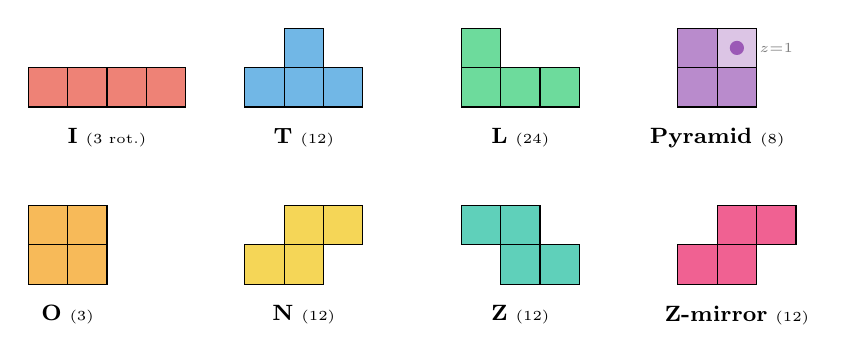
\begin{tikzpicture}[scale=0.50]
    % ── Row 1: I  T  L  Pyramid
    \begin{scope}[xshift=0cm]
      \sqfill{0}{0}{piece-I!70}\sqfill{1}{0}{piece-I!70}
      \sqfill{2}{0}{piece-I!70}\sqfill{3}{0}{piece-I!70}
      \node[below, font=\footnotesize] at (2,-0.3) {\textbf{I} \tiny(3 rot.)};
    \end{scope}
    \begin{scope}[xshift=5.5cm]
      \sqfill{0}{0}{piece-T!70}\sqfill{1}{0}{piece-T!70}
      \sqfill{2}{0}{piece-T!70}\sqfill{1}{1}{piece-T!70}
      \node[below, font=\footnotesize] at (1.5,-0.3) {\textbf{T} \tiny(12)};
    \end{scope}
    \begin{scope}[xshift=11cm]
      \sqfill{0}{0}{piece-L!70}\sqfill{1}{0}{piece-L!70}
      \sqfill{2}{0}{piece-L!70}\sqfill{0}{1}{piece-L!70}
      \node[below, font=\footnotesize] at (1.5,-0.3) {\textbf{L} \tiny(24)};
    \end{scope}
    \begin{scope}[xshift=16.5cm]
      \sqfill{0}{0}{piece-Pyr!70}\sqfill{1}{0}{piece-Pyr!70}
      \sqfill{0}{1}{piece-Pyr!70}
      \fill[piece-Pyr!35, draw=black, line width=0.4pt]
            (1,1) rectangle +(1,1);
      \fill[piece-Pyr] (1.5,1.5) circle (0.18);
      \node[font=\tiny, gray] at (2.5,1.5) {$z{=}1$};
      \node[below, font=\footnotesize] at (1,-0.3) {\textbf{Pyramid} \tiny(8)};
    \end{scope}
    % ── Row 2: O  N  Z  Z-mirror
    \begin{scope}[xshift=0cm, yshift=-4.5cm]
      \sqfill{0}{0}{piece-O!70}\sqfill{1}{0}{piece-O!70}
      \sqfill{0}{1}{piece-O!70}\sqfill{1}{1}{piece-O!70}
      \node[below, font=\footnotesize] at (1,-0.3) {\textbf{O} \tiny(3)};
    \end{scope}
    \begin{scope}[xshift=5.5cm, yshift=-4.5cm]
      \sqfill{0}{0}{piece-N!70}\sqfill{1}{0}{piece-N!70}
      \sqfill{1}{1}{piece-N!70}\sqfill{2}{1}{piece-N!70}
      \node[below, font=\footnotesize] at (1.5,-0.3) {\textbf{N} \tiny(12)};
    \end{scope}
    \begin{scope}[xshift=11cm, yshift=-4.5cm]
      \sqfill{0}{1}{piece-Z!70}\sqfill{1}{1}{piece-Z!70}
      \sqfill{1}{0}{piece-Z!70}\sqfill{2}{0}{piece-Z!70}
      \node[below, font=\footnotesize] at (1.5,-0.3) {\textbf{Z} \tiny(12)};
    \end{scope}
    \begin{scope}[xshift=16.5cm, yshift=-4.5cm]
      \sqfill{0}{0}{piece-Zm!70}\sqfill{1}{0}{piece-Zm!70}
      \sqfill{1}{1}{piece-Zm!70}\sqfill{2}{1}{piece-Zm!70}
      \node[below, font=\footnotesize] at (1.5,-0.3) {\textbf{Z-mirror} \tiny(12)};
    \end{scope}
  \end{tikzpicture}

  \vspace{0.3cm}
  \begin{columns}[T]
    \column{0.48\textwidth}
      {\small\color{umons-blue} \textbf{Total: 86 distinct orientations}}\\
      {\footnotesize 7 planar + 1 non-planar (Pyramid)}
    \column{0.48\textwidth}
      {\footnotesize
       \textbf{Pyramid} is the only truly 3D piece: 3 ground-floor cubes
       $+$ 1 elevated cube at $z=1$ (shown as filled dot).}
  \end{columns}
\end{frame}

% ── Slide 4 ───────────────────────────────────────────────────────────────────
\begin{frame}{Slide 4 --- Rotations \& Symmetry \hfill \mohamed}
  \begin{columns}[T]
    \column{0.50\textwidth}
      \begin{block}{How rotations are computed}
        Python applies each of the \textbf{24 rotation matrices}
        (the group $S_4$) to the base offsets $(DX,DY,DZ)$,
        deduplicates, and exports to \texttt{tetracubes.lp}:
        \begin{center}
        {\ttfamily\scriptsize
          cube("I",\,1,\,0,0,0). cube("I",\,1,\,0,0,1).\\
          cube("I",\,1,\,0,0,2). cube("I",\,1,\,0,0,3).}
        \end{center}
        {\footnotesize All 86 orientations generated this way}
      \end{block}

    \column{0.47\textwidth}
      \begin{block}{Rotation count by symmetry}
        \renewcommand{\arraystretch}{1.2}
        \begin{tabular}{@{}lcc@{}}
          \toprule
          \textbf{Piece} & \textbf{Rot.} & \textbf{Why} \\
          \midrule
          \textcolor{piece-I}{\textbf{I}},
          \textcolor{piece-O}{\textbf{O}} & 3 & High symmetry \\[2pt]
          \textcolor{piece-T}{\textbf{T}},
          \textcolor{piece-N}{\textbf{N}},
          \textcolor{piece-Z}{\textbf{Z}},
          \textcolor{piece-Zm}{\textbf{Zm}} & 12 & Partial sym. \\[2pt]
          \textcolor{piece-Pyr}{\textbf{Pyramid}} & 8 & Octahedral \\[2pt]
          \textcolor{piece-L}{\textbf{L}} & \textbf{24} & \textbf{No symmetry} \\
          \midrule
          Total & \textbf{86} & \\
          \bottomrule
        \end{tabular}
      \end{block}
  \end{columns}

  \vspace{0.3cm}
  \begin{alertblock}{Key fact}
    \textbf{L} has 24 orientations because it is \emph{chiral and asymmetric}
    --- every rotation matrix gives a new distinct placement.
    \textbf{Z} and \textbf{Z-mirror} are mirror images; neither is a rotation of the other.
  \end{alertblock}
\end{frame}

% ══════════════════════════════════════════════════════════════════════════════
% PART 2
% ══════════════════════════════════════════════════════════════════════════════

\begin{frame}[plain]
  \begin{tikzpicture}[remember picture, overlay]
    \fill[t-blue!80] (current page.center) circle (4.5cm);
    \node[text=white, font=\LARGE\bfseries, align=center]
          at (current page.center)
          {Part 2\\[8pt]\Large Volume Configurations};
  \end{tikzpicture}
\end{frame}

% ── Slide 5 ───────────────────────────────────────────────────────────────────
\begin{frame}[fragile]{Slide 5 --- The ``Shape-Agnostic'' Vision \hfill \abdelhadi}
  \begin{columns}[T]
    \column{0.52\textwidth}
      \begin{block}{Old approach (hardcoded bounds)}
        {\ttfamily\small cell(X,Y,Z) :- X=0..3, Y=0..1, Z=0..3.}\\[4pt]
        {\footnotesize Only works for a $4\times2\times4$ box.
         Every new shape requires new solver code.}
      \end{block}

      \vspace{0.4cm}
      \begin{exampleblock}{New approach: explicit \texttt{cell/3} listing}
        \begin{lstlisting}[style=aspstyle]
% T-shape: bar + stem, depth 2
cell(X,Y,Z) :- X=0..3, Y=4..5, Z=0..1.
cell(X,Y,Z) :- X=1..2, Y=0..3, Z=0..1.
        \end{lstlisting}
        {\footnotesize \texttt{puzzle.lp} only reads \texttt{cell/3}.
         Swap this file $\Rightarrow$ new shape, \textbf{same solver}.}
      \end{exampleblock}

    \column{0.44\textwidth}
      \centering
      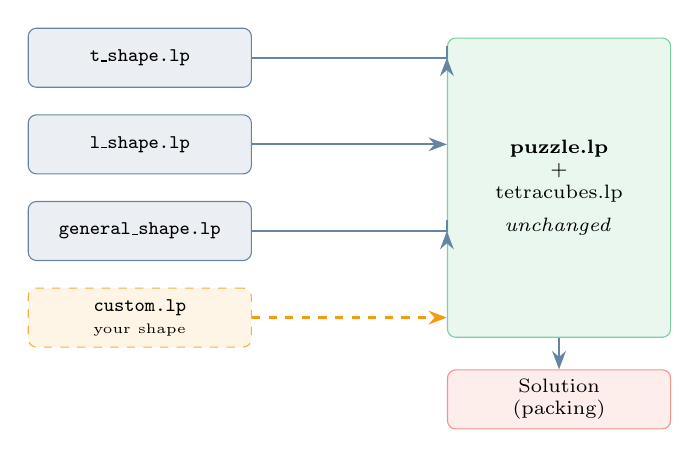
\begin{tikzpicture}[node distance=0.4cm,
        box/.style={rectangle, rounded corners=3pt, draw=umons-blue!60,
                    fill=umons-blue!8, minimum height=0.75cm,
                    text width=2.6cm, align=center, font=\scriptsize},
        arr/.style={-Stealth, thick, umons-blue!60}]
        \node[box] (s1) at (0, 4.2) {\texttt{t\_shape.lp}};
        \node[box] (s2) at (0, 3.1) {\texttt{l\_shape.lp}};
        \node[box] (s3) at (0, 2.0) {\texttt{general\_shape.lp}};
        \node[box, dashed, draw=hint-gold!80, fill=hint-gold!10]
              (sn) at (0, 0.9) {\texttt{custom.lp}\\{\tiny your shape}};
        \node[box, right=1.0cm of s2, fill=asp-green!10, draw=asp-green!60,
              minimum height=3.8cm, text width=2.6cm]
              (engine) at (2.9, 2.55)
              {\textbf{puzzle.lp}\\+\\tetracubes.lp\\[4pt]\textit{unchanged}};
        \node[box, below=0.4cm of engine, fill=l-red!10, draw=l-red!60]
              (out) {Solution\\(packing)};
        \draw[arr] (s1.east) -| (engine.north west|-s1.east)
                   -- (engine.north west|-s1.east);
        \draw[arr] (s2.east) -- (engine.west|-s2.east);
        \draw[arr] (s3.east) -| (engine.west|-s3.east);
        \draw[arr, dashed, hint-gold] (sn.east) -- (engine.west|-sn.east);
        \draw[arr] (engine.south) -- (out.north);
      \end{tikzpicture}
  \end{columns}
\end{frame}

% ── Slide 6 ───────────────────────────────────────────────────────────────────
\begin{frame}[fragile]{Slide 6 --- Configuration 1: T-Shape \hfill \mohamed}
  \begin{columns}[T]
    \column{0.45\textwidth}
      \begin{block}{Geometry: bar $\cup$ stem, depth 2}
        $\underbrace{\{0..3\}\times\{4..5\}}_{\text{bar}} \cup
         \underbrace{\{1..2\}\times\{0..3\}}_{\text{stem}}
         \times\{0,1\}$
      \end{block}
      \vspace{0.1cm}
      \begin{block}{Cell count \checkmark}
        Bar: $4\times2=8$/layer \quad Stem: $2\times4=8$/layer\\
        No overlap ($y_{\text{bar}}\geq4$, $y_{\text{stem}}\leq3$)\\
        Total: $16\times2=\mathbf{32}$
      \end{block}
      \vspace{0.1cm}
      \begin{lstlisting}[style=aspstyle, title=t\_shape.lp]
cell(X,Y,Z) :- X=0..3, Y=4..5, Z=0..1.
cell(X,Y,Z) :- X=1..2, Y=0..3, Z=0..1.
      \end{lstlisting}

    \column{0.50\textwidth}
      \centering
      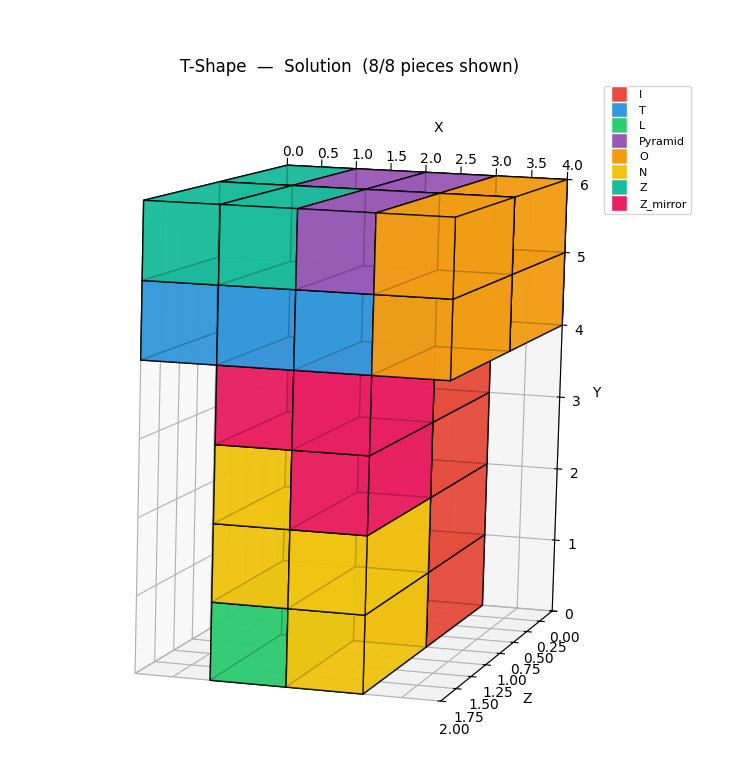
\includegraphics[width=\linewidth]{img_slide6}
      {\scriptsize\color{gray} 3D visualisation --- T-Shape solution (8/8 pieces)}
  \end{columns}
\end{frame}

% ── Slide 7 ───────────────────────────────────────────────────────────────────
\begin{frame}[fragile]{Slide 7 --- Configuration 2: L-Shape \hfill \abdelhadi}
  \begin{columns}[T]
    \column{0.45\textwidth}
      \begin{block}{Geometry: $4\times5$ minus $2\times2$ corner}
        $[0..3]\times[0..4]\;\setminus\;\{x\!\in\!\{2,3\},\,y\!\in\!\{3,4\}\}$
        $\times\{0,1\}$
      \end{block}
      \vspace{0.1cm}
      \begin{alertblock}{Non-convex boundary}
        This shape has a \textbf{concave corner}. The solver handles
        it identically --- no change to the engine needed.
      \end{alertblock}
      \vspace{0.1cm}
      \begin{lstlisting}[style=aspstyle, title=l\_shape.lp]
% Left columns: full height
cell(X,Y,Z) :- X=0..1, Y=0..4, Z=0..1.
% Right columns: bottom 3 rows only
cell(X,Y,Z) :- X=2..3, Y=0..2, Z=0..1.
      \end{lstlisting}

    \column{0.50\textwidth}
      \centering
      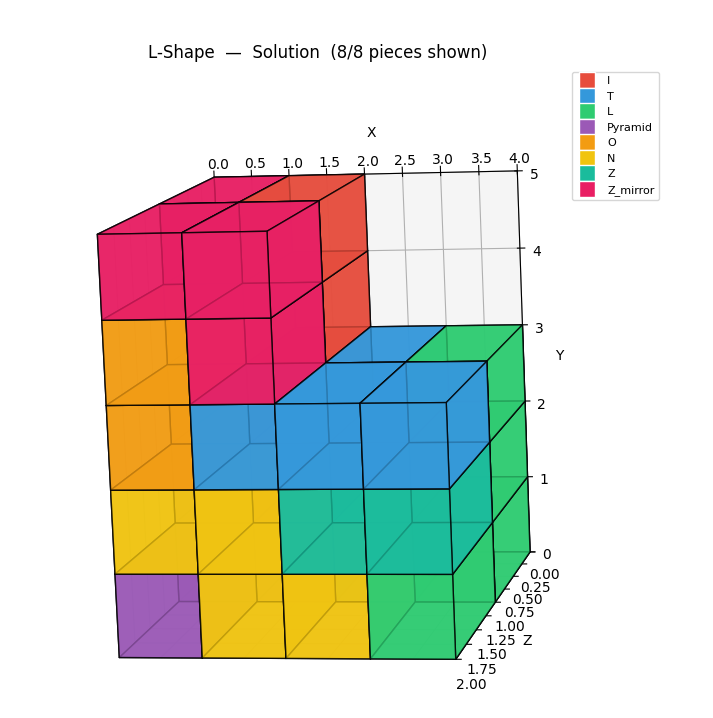
\includegraphics[width=\linewidth]{img_slide7}
      {\scriptsize\color{gray} 3D visualisation --- L-Shape solution (8/8 pieces)}
  \end{columns}
\end{frame}

% ── Slide 8 ───────────────────────────────────────────────────────────────────
\begin{frame}[fragile]{Slide 8 --- Configuration 3: Plus/Cross Shape \hfill \mohamed}
  \begin{columns}[T]
    \column{0.45\textwidth}
      \begin{block}{Geometry: body + arms, depth 2}
        $\underbrace{\{0..3\}\times\{1..3\}}_{\text{body}} \cup
         \underbrace{\{1..2\}\times\{4\}}_{\text{top}} \cup
         \underbrace{\{1..2\}\times\{0\}}_{\text{bottom}}
         \times\{0,1\}$
      \end{block}
      \vspace{0.1cm}
      \begin{block}{Cell count \checkmark}
        Body: $12$/layer \quad Arms: $4$/layer\\
        Total: $16\times2=\mathbf{32}$
      \end{block}
      \vspace{0.1cm}
      \begin{lstlisting}[style=aspstyle, title=general\_shape.lp]
cell(X,Y,Z) :- X=0..3, Y=1..3, Z=0..1.
cell(X,Y,Z) :- X=1..2, Y=4..4, Z=0..1.
cell(X,Y,Z) :- X=1..2, Y=0..0, Z=0..1.
      \end{lstlisting}

    \column{0.50\textwidth}
      \centering
      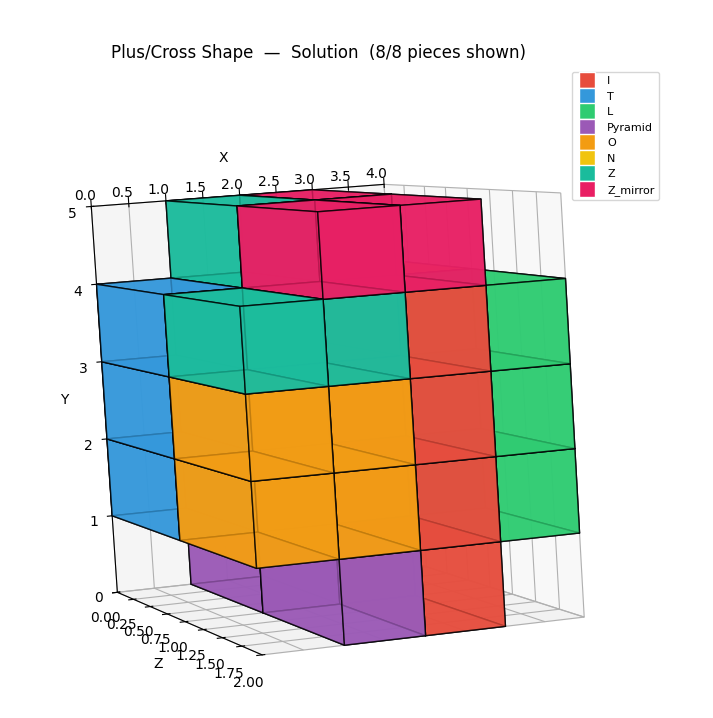
\includegraphics[width=\linewidth]{img_slide8}
      {\scriptsize\color{gray} 3D visualisation --- Plus/Cross solution (8/8 pieces)}
  \end{columns}
\end{frame}

% ══════════════════════════════════════════════════════════════════════════════
% PART 3
% ══════════════════════════════════════════════════════════════════════════════

\begin{frame}[plain]
  \begin{tikzpicture}[remember picture, overlay]
    \fill[asp-green!80] (current page.center) circle (4.5cm);
    \node[text=white, font=\LARGE\bfseries, align=center]
          at (current page.center)
          {Part 3\\[8pt]\Large ASP Modelling \& Logic};
  \end{tikzpicture}
\end{frame}

% ── Slide 9 ───────────────────────────────────────────────────────────────────
\begin{frame}[fragile]{Slide 9 --- Core Architecture: The \texttt{cell/3} Abstraction \hfill \abdelhadi}
  \begin{columns}[T]
    \column{0.52\textwidth}
      \begin{block}{The central design insight}
        The entire solver makes \textbf{one} assumption about the target:
        valid positions are ground atoms of \texttt{cell(X,Y,Z)}.\\[6pt]
        \emph{Logic and geometry are completely decoupled.}
      \end{block}

      \vspace{0.3cm}
      {\small
        \begin{tabular}{@{}lp{4.5cm}@{}}
          \toprule
          \textbf{File} & \textbf{Responsibility} \\
          \midrule
          \texttt{*\_shape.lp} & declares which cells exist \\
          \texttt{puzzle.lp}   & placement / coverage rules \\
          \texttt{tetracubes.lp} & piece rotation offsets \\
          \bottomrule
        \end{tabular}
      }

      \vspace{0.3cm}
      \begin{exampleblock}{Consequence}
        A new shape = a new \texttt{.lp} file.
        \textbf{Nothing else changes.}
      \end{exampleblock}

    \column{0.44\textwidth}
      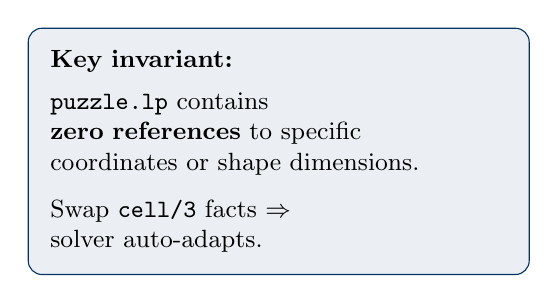
\begin{tikzpicture}
        \node[draw=umons-blue, rounded corners=5pt,
              fill=umons-blue!8, text width=5.8cm,
              align=left, font=\small, inner sep=8pt]{%
          \textbf{Key invariant:}\\[4pt]
          \texttt{puzzle.lp} contains\\
          \textbf{zero references} to specific\\
          coordinates or shape dimensions.\\[6pt]
          Swap \texttt{cell/3} facts $\Rightarrow$\\
          solver auto-adapts.};
      \end{tikzpicture}

      \vspace{0.4cm}
      \begin{lstlisting}[style=bashstyle]
# Solve T
clingo t_shape.lp puzzle.lp tetracubes.lp

# Solve Plus -- same engine!
clingo general_shape.lp puzzle.lp tetracubes.lp
      \end{lstlisting}
  \end{columns}
\end{frame}

% ── Slide 10 ──────────────────────────────────────────────────────────────────
\begin{frame}[fragile]{Slide 10 --- ASP Rules: Placement \& Boundary \hfill \mohamed}
  \begin{columns}[T]
    \column{0.52\textwidth}
      \begin{block}{Rule 1 --- One placement per piece}
        \begin{lstlisting}[style=aspstyle]
1 { position(P,R,X,Y,Z)
  : cell(X,Y,Z),
    validOrientation(Type,R) } 1 :-
  tetracubeID(P), assignType(P,Type).
        \end{lstlisting}
        {\footnotesize Exactly one anchor $(X,Y,Z)$ + rotation $R$
        per piece. Anchor must be a valid cell.}
      \end{block}

      \vspace{0.3cm}
      \begin{block}{Deriving occupied cells}
        \begin{lstlisting}[style=aspstyle]
occupied(P, X+DX, Y+DY, Z+DZ) :-
  position(P,R,X,Y,Z),
  assignType(P,Type),
  cube(Type,R,DX,DY,DZ).
        \end{lstlisting}
        {\footnotesize All 4 cells = anchor $+$ offsets from
        \texttt{tetracubes.lp}.}
      \end{block}

    \column{0.45\textwidth}
      \begin{alertblock}{Rule 2 --- Boundary constraint}
        \begin{lstlisting}[style=aspstyle]
:- position(P,R,X,Y,Z),
   assignType(P,Type),
   cube(Type,R,DX,DY,DZ),
   not cell(X+DX, Y+DY, Z+DZ).
        \end{lstlisting}
        {\footnotesize Every cell of a piece must be inside
        the \texttt{cell/3} set. Pieces cannot "stick out".}
      \end{alertblock}

      \vspace{0.5cm}
      \centering
      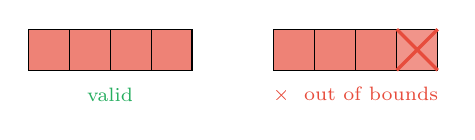
\begin{tikzpicture}[scale=0.52]
        % Valid placement (I piece inside shape)
        \sqfill{0}{0}{t-blue!25}\sqfill{1}{0}{t-blue!25}
        \sqfill{2}{0}{t-blue!25}\sqfill{3}{0}{t-blue!25}
        \sqfill{0}{0}{piece-I!70}\sqfill{1}{0}{piece-I!70}
        \sqfill{2}{0}{piece-I!70}\sqfill{3}{0}{piece-I!70}
        \node[font=\scriptsize, asp-green] at (2,-0.6) {\checkmark valid};
        % Invalid (piece overflows)
        \sqfill{6}{0}{t-blue!25}\sqfill{7}{0}{t-blue!25}
        \sqfill{8}{0}{t-blue!25}
        \sqfill{6}{0}{piece-I!70}\sqfill{7}{0}{piece-I!70}
        \sqfill{8}{0}{piece-I!70}
        \fill[l-red!60, draw=black, line width=0.5pt]
              (9,0) rectangle +(1,1);
        \draw[l-red, very thick] (9,0)--(10,1) (10,0)--(9,1);
        \node[font=\scriptsize, l-red] at (8,-0.6) {\texttimes\; out of bounds};
      \end{tikzpicture}
  \end{columns}
\end{frame}

% ── Slide 11 ──────────────────────────────────────────────────────────────────
\begin{frame}[fragile]{Slide 11 --- ASP Rules: Non-Overlap \& Coverage \hfill \abdelhadi}
  \begin{columns}[T]
    \column{0.50\textwidth}
      \begin{alertblock}{Rule 3 --- Non-overlap}
        \begin{lstlisting}[style=aspstyle]
:- occupied(P1,X,Y,Z),
   occupied(P2,X,Y,Z),
   P1 != P2.
        \end{lstlisting}
        {\footnotesize Two distinct pieces cannot share
        the same unit cube $(X,Y,Z)$.}
      \end{alertblock}

      \vspace{0.4cm}
      \begin{alertblock}{Rule 4 --- Full coverage}
        \begin{lstlisting}[style=aspstyle]
cellOccupied(X,Y,Z) :-
  occupied(P,X,Y,Z), tetracubeID(P).

:- cell(X,Y,Z),
   not cellOccupied(X,Y,Z).
        \end{lstlisting}
        {\footnotesize Every cell declared by \texttt{cell/3} must
        be covered by exactly one piece.}
      \end{alertblock}

    \column{0.47\textwidth}
      \begin{block}{The four rules together}
        \renewcommand{\arraystretch}{1.2}
        \begin{tabular}{@{}cl@{}}
          \toprule
          \textbf{Rule} & \textbf{Guarantee} \\
          \midrule
          1 & Each piece placed exactly once \\
          2 & No piece goes outside the shape \\
          3 & No two pieces share a cell \\
          4 & All 32 cells are covered \\
          \bottomrule
        \end{tabular}
      \end{block}

      \vspace{0.4cm}
      \begin{exampleblock}{What Clingo does}
        Searches for an assignment satisfying
        all 4 rules simultaneously --- a \textbf{perfect tiling}.\\[4pt]
        No solution exists $\Rightarrow$ \texttt{UNSATISFIABLE}.\\
        Solution exists $\Rightarrow$ answer set = packing.
      \end{exampleblock}
  \end{columns}
\end{frame}

% ── Slide 12 ──────────────────────────────────────────────────────────────────
\begin{frame}[fragile]{Slide 12 --- Hint System \& Difficulty Levels \hfill \mohamed}
  \begin{columns}[T]
    \column{0.50\textwidth}
      \begin{block}{Hint generation in ASP}
        \begin{lstlisting}[style=aspstyle]
#const num_hints = 5.

% Select exactly num_hints pieces to reveal
{ hint(P) : tetracubeID(P) } num_hints.
:- num_hints != #count{P : hint(P)}.

% Bias toward diverse selection
#heuristic hint(P) : tetracubeID(P).
  [seed@3, false]
        \end{lstlisting}
        {\footnotesize Override at runtime:\\
        \texttt{clingo ... -c num\_hints=3}}
      \end{block}

    \column{0.47\textwidth}
      \begin{block}{Difficulty levels}
        \renewcommand{\arraystretch}{1.2}
        \begin{tabular}{@{}ccc@{}}
          \toprule
          \textbf{Hints} & \textbf{Hidden} & \textbf{Level} \\
          \midrule
          7 & 1 & Very Easy \\
          5--6 & 2--3 & Easy \\
          3--4 & 4--5 & Medium \\
          1--2 & 6--7 & Hard \\
          0   & 8   & Harder \\
          \bottomrule
        \end{tabular}
      \end{block}

      \vspace{0.2cm}
      {\footnotesize
        \textbf{Hints} = pre-placed pieces (given to player).\\
        \textbf{Hidden} = pieces the player must place.}

      \vspace{0.1cm}
      \centering
      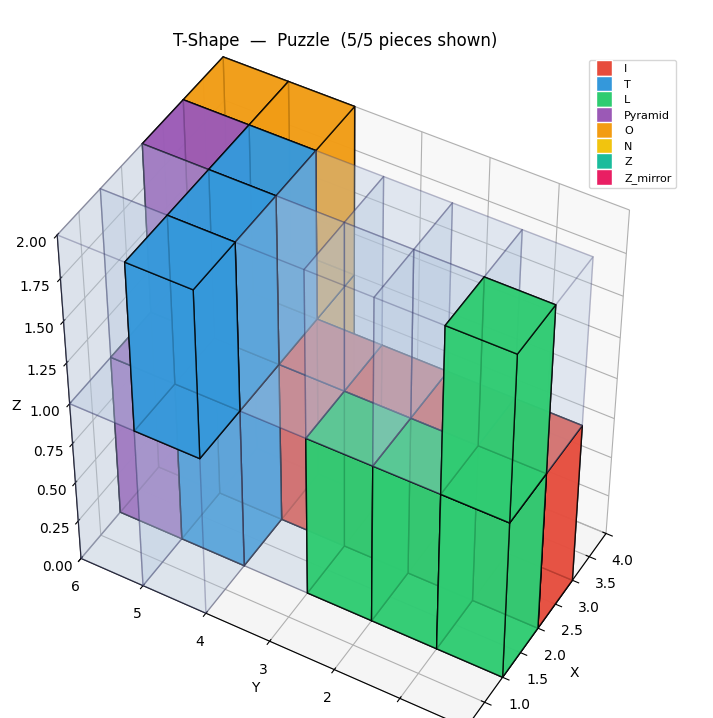
\includegraphics[height=2.4cm, keepaspectratio]{img_slide12}\\
      {\scriptsize\color{gray} Puzzle view: 5 hints shown, 3 hidden}
  \end{columns}
\end{frame}

% ══════════════════════════════════════════════════════════════════════════════
% PART 4
% ══════════════════════════════════════════════════════════════════════════════

\begin{frame}[plain]
  \begin{tikzpicture}[remember picture, overlay]
    \fill[plus-purple!80] (current page.center) circle (4.5cm);
    \node[text=white, font=\LARGE\bfseries, align=center]
          at (current page.center)
          {Part 4\\[8pt]\Large Generalisation \& Results};
  \end{tikzpicture}
\end{frame}

% ── Slide 13 ──────────────────────────────────────────────────────────────────
\begin{frame}[fragile]{Slide 13 --- Random Shape Generation \hfill \abdelhadi}
  \begin{columns}[T]
    \column{0.50\textwidth}
      \begin{block}{\texttt{random\_puzzle.py} --- Eden growth model}
        \begin{enumerate}
          \item Start from one seed cell
          \item Maintain a \textbf{frontier}: all face-neighbours
                of the current shape
          \item Randomly pick one frontier cell, add it
          \item Repeat until \textbf{32 cells} reached
          \item Guarantees connectivity by construction
        \end{enumerate}
      \end{block}

      \vspace{0.2cm}
      \begin{lstlisting}[style=bashstyle]
# Random 2D slab (default, reliable)
python random_puzzle.py

# Fixed seed, hard puzzle, ASCII art
python random_puzzle.py --seed 42 \
       --hints 2 --show-shape

# True 3D polycube
python random_puzzle.py --mode 3d
      \end{lstlisting}

    \column{0.47\textwidth}
      \centering
      \includegraphics[width=\linewidth]{img_slide13}
  \end{columns}
\end{frame}

% ── Slide 14 ──────────────────────────────────────────────────────────────────
\begin{frame}{Slide 14 --- Solving the ``True 3D'' Challenge \hfill \mohamed}
  \begin{columns}[T]
    \column{0.50\textwidth}
      \begin{block}{Two generation modes}
        \renewcommand{\arraystretch}{1.2}
        \begin{tabular}{@{}lll@{}}
          \toprule
          \textbf{Mode} & \textbf{Growth} & \textbf{Reliability} \\
          \midrule
          2D (default) & $\pm x,\pm y$, depth=2 & High \\
          3D (\texttt{--mode 3d}) & $\pm x,\pm y,\pm z$ & Low--Med \\
          \bottomrule
        \end{tabular}
      \end{block}

      \vspace{0.15cm}
      \begin{exampleblock}{Why 2D is reliable}
        Depth-2 slabs give every cell $\geq 2$ z-neighbours ---
        enough room for any tetracube. Solve: $<30$\,ms.
      \end{exampleblock}

      \vspace{0.15cm}
      \begin{alertblock}{Why 3D can fail}
        Eden 3D creates \textbf{thin tendrils}: dead-end cells
        where no tetracube fits without leaving a gap.
        Script retries up to 50 times automatically.
      \end{alertblock}

    \column{0.47\textwidth}
      \centering
      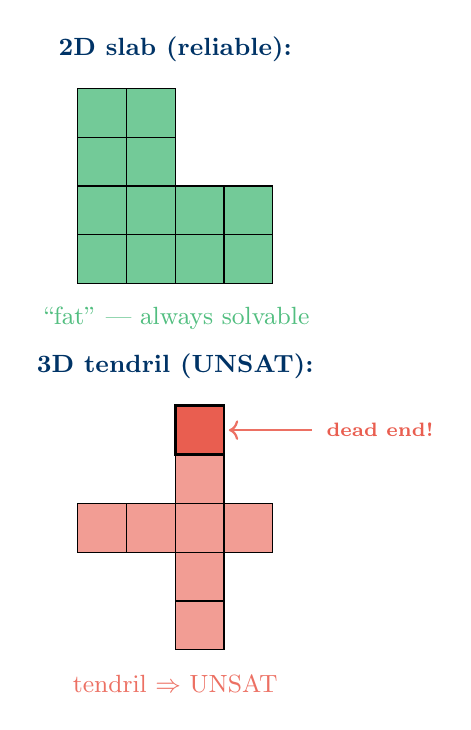
\begin{tikzpicture}[scale=0.62]
        % ── 2D slab (fat, reliable) ──
        \node[font=\small\bfseries, umons-blue] at (2.0, 4.8)
              {2D slab (reliable):};
        % L-shape: full 4 wide bottom 2 rows, left 2 cols extend higher
        \sqfill{0}{0}{asp-green!65}\sqfill{1}{0}{asp-green!65}
        \sqfill{2}{0}{asp-green!65}\sqfill{3}{0}{asp-green!65}
        \sqfill{0}{1}{asp-green!65}\sqfill{1}{1}{asp-green!65}
        \sqfill{2}{1}{asp-green!65}\sqfill{3}{1}{asp-green!65}
        \sqfill{0}{2}{asp-green!65}\sqfill{1}{2}{asp-green!65}
        \sqfill{0}{3}{asp-green!65}\sqfill{1}{3}{asp-green!65}
        \node[font=\small, asp-green!80, align=center] at (2.0,-0.7)
              {``fat'' --- always solvable};

        % ── 3D tendril (UNSAT) ──
        \begin{scope}[yshift=-7.5cm]
          \node[font=\small\bfseries, umons-blue] at (2.0, 5.8)
                {3D tendril (UNSAT):};
          % Cross/winding shape
          \sqfill{2}{0}{l-red!55}\sqfill{2}{1}{l-red!55}
          \sqfill{0}{2}{l-red!55}\sqfill{1}{2}{l-red!55}
          \sqfill{2}{2}{l-red!55}\sqfill{3}{2}{l-red!55}
          \sqfill{2}{3}{l-red!55}
          % Dead-end cell at top (darker)
          \fill[l-red!90, draw=black, line width=1pt]
                (2,4) rectangle +(1,1);
          % Arrow + label
          \draw[->, l-red!80, thick] (4.8,4.5) -- (3.1,4.5);
          \node[font=\scriptsize\bfseries, l-red!90, anchor=west] at (4.9,4.5)
                {dead end!};
          \node[font=\small, l-red!80, align=center] at (2.0,-0.7)
                {tendril $\Rightarrow$ UNSAT};
        \end{scope}
      \end{tikzpicture}
  \end{columns}
\end{frame}

% ── Slide 15 ──────────────────────────────────────────────────────────────────
\begin{frame}{Slide 15 --- Verification \& Complexity \hfill \abdelhadi}
  \begin{columns}[T]
    \column{0.50\textwidth}
      \begin{block}{\texttt{verify.py} --- 6 independent checks}
        \begin{enumerate}
          \item Exactly 8 pieces placed
          \item Each piece has exactly 4 cells
          \item All cells within the declared shape
          \item No two pieces share a cell
          \item Every shape cell is covered
          \item Each piece type appears exactly once
        \end{enumerate}
        {\footnotesize Reconstructs and checks the solution
        \emph{without trusting Clingo's output}.}
      \end{block}

    \column{0.47\textwidth}
      \begin{block}{Performance (all shapes solved in $<60$\,ms)}
        \renewcommand{\arraystretch}{1.2}
        \begin{tabular}{@{}lcc@{}}
          \toprule
          \textbf{Shape} & \textbf{Time} & \textbf{Result} \\
          \midrule
          T-shape     & $<50$\,ms & \textcolor{asp-green}{\textbf{SAT}} \\
          L-shape     & $<50$\,ms & \textcolor{asp-green}{\textbf{SAT}} \\
          Plus/Cross  & $\approx35$\,ms & \textcolor{asp-green}{\textbf{SAT}} \\
          Rnd. 2D slab & $<30$\,ms & \textcolor{asp-green}{\textbf{SAT}} \\
          Rnd. 3D     & $1$--$60$\,ms & varies \\
          \bottomrule
        \end{tabular}
      \end{block}
  \end{columns}
\end{frame}

% ── Slide 16 ──────────────────────────────────────────────────────────────────
\begin{frame}{Slide 16 --- Conclusion \& Future Work \hfill \mohamed}
  \begin{columns}[T]
    \column{0.50\textwidth}
      \begin{block}{What we proved}
        \begin{itemize}
          \item Non-rectangular 3D volumes \textbf{are} perfectly
                tileable by the 8 standard tetracubes
          \item A single \texttt{cell/3} predicate suffices to define
                \emph{any} target volume for the solver
          \item The same ASP engine solves T, L, Plus/Cross, and
                random polycubes \textbf{without modification}
          \item All solutions pass 6 independent correctness checks
        \end{itemize}
      \end{block}
  \end{columns}

  \vspace{0.4cm}
  \centering
  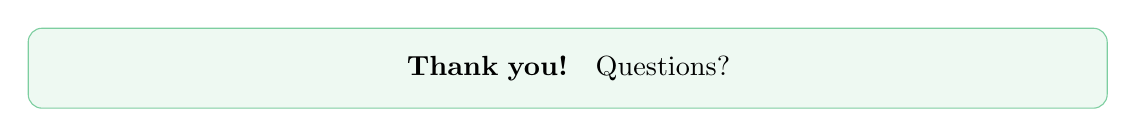
\begin{tikzpicture}
    \node[draw=asp-green!60, fill=asp-green!8, rounded corners=5pt,
          text width=13cm, align=center, font=\normalsize, inner sep=10pt]{%
      \textbf{Thank you!}\quad Questions?\\[4pt]
      };
  \end{tikzpicture}
\end{frame}

\end{document}
